\documentclass[12pt]{article}

\usepackage[T1]{fontenc}
\usepackage[english,greek]{babel}
%\usepackage{tgschola}
\newcommand {\lat}{\latintext}
\usepackage{algorithm}
\usepackage{algorithmic}
\usepackage{kerkis} 

%\usepackage{mathptmx}
\usepackage{gensymb}


\usepackage[dvipsnames]{xcolor}
\usepackage{color}

\definecolor{c1}{rgb}{0.9,0,0.3}
\definecolor{c2}{rgb}{0.65,0,0.8}
\definecolor{c3}{rgb}{1,1,0.65}
\definecolor{c4}{rgb}{0.94,0.65,0.30}
\definecolor{c5}{rgb}{0.90,0.65,0}
\definecolor{c6}{rgb}{0.50,1,0}
\definecolor{c7}{rgb}{0,0.65,0}
\definecolor{c8}{rgb}{0.65,0,0.8}
\definecolor{c9}{rgb}{0.50,0.61,0.14}
\definecolor{c10}{rgb}{0.90,0.80,0.30}
\definecolor{c11}{rgb}{0.90,0.90,0.30}
\definecolor{c12}{rgb}{0.80,0.80,0.80}
\definecolor{c13}{rgb}{0.30,0.30,1}
\definecolor{c14}{rgb}{0.50,0.94,0.90}

\usepackage{cancel}
\usepackage{graphicx} % for images
\graphicspath{ {./images/} } % images path




\usepackage[top=0.5in, bottom=1in, left=1.2in, right=1in]{geometry}
\pagestyle{plain}
\linespread{1.2} 

\usepackage{titlesec}

\titleformat{\section}
  {\normalfont\fontsize{22}{15}\bfseries}{\thesection}{1em}{}

\usepackage{hyperref}
\hypersetup{
    colorlinks=true,
    linkcolor=blue,
    filecolor=magenta,      
    urlcolor=cyan,
    pdftitle={Overleaf Example},
    pdfpagemode=FullScreen,
    }

% For bibliography %
\usepackage{biblatex} %Imports biblatex package
\addbibresource{bibliography.bib} %Import the bibliography file

\usepackage{tikz}

\newcommand{\pair}[2]{\langle #1,\, #2 \rangle}
\newcommand{\triple}[3]{\langle #1,\, #2,\, #3 \rangle}

\DeclareSymbolFont{matha}{OML}{txmi}{m}{it}% txfonts
\DeclareMathSymbol{\varv}{\mathord}{matha}{118}

\usepackage{tabularx,ragged2e,booktabs,caption}
\newcolumntype{C}[1]{>{\Centering}m{#1}}
\renewcommand\tabularxcolumn[1]{C{#1}}
\renewcommand{\textfraction}{0.05} 

\usepackage{blkarray}
\usepackage{amssymb}
\usepackage{amsmath}
\DeclareMathOperator*{\argmax}{arg\,max}
\DeclareMathOperator*{\argmin}{arg\,min}
\newcommand{\Mod}[1]{\ (\mathrm{mod}\ #1)}
\usepackage{mathtools}



%%%%%% FOR TABLES %%%%%%%%%%
\usepackage{tabularx,ragged2e,booktabs,caption}
%\newcolumntype{C}[1]{>{\Centering}m{#1}}
\renewcommand\tabularxcolumn[1]{C{#1}}
\renewcommand{\textfraction}{0.05} 
\renewcommand{\arraystretch}{1.1}
\newcommand\norm[1]{\lVert#1\rVert}
\newcommand{\diam}{\text{diam}}
\DeclareMathOperator{\EX}{\mathbb{E}}% expected value

\usepackage{algorithm}
\usepackage{algorithmic}
\usepackage{authblk}
\usepackage{amsthm}
\usepackage{bbm}
\usepackage{tabularx}

\newcommand{\thedate}{\today}

\newtheorem{theorem}{Theorem}
\theoremstyle{definition}
\newtheorem{definition}{Definition}
\newtheorem{corollary}{Corollary}[theorem]

\begin{document}

\begin{titlepage}
\begin{center}

\begin{figure}[h!]
    \centering
\includegraphics[width=0.7\textwidth]{images/nkualogo.png}
\end{figure}

\textnormal{ \LARGE{Τμήμα Πληροφορικής και Τηλεπικοινωνιών\\ }}
\end{center}
\vspace{25mm}

\begin{center}
\textsc{\LARGE Τεχνητή Νοημοσύνη Ι\\}
\end{center}


\vspace{8mm}
\begin{center}
	\fontsize{8mm}{5mm}\selectfont 
	
    \textup{\emph{Πρώτη Εργασία}}\\
    
    \textup{\emph{Θεωρητικές Ασκήσεις}}\\

	\vspace{5mm}

\end{center}
\vspace{8mm}

\vfill

\noindent \textsc{\Large \emph{Συγγραφή: Χρήστος Νίκου}}\\
\textsc{\Large \emph{ΑΜ: 1115201800330}}\\
\vspace{3mm}


\vspace{2mm}

\begin{center}
\vspace{2cm}

\LARGE {\thedate}    
\end{center}

\end{titlepage}

\section*{Πρόβλημα 2}

\bf Απάντηση:\, \normalfont Εφ' όσον ο κόμβος στόχου βρίσκεται σε βάθος $g\leq d$ ο αλγόριθμος πρώτα σε βάθος με επαναληπτική εκβάθυνση θα πραγματοποιήσει ακριβώς $g$ φορές τον αλγόριθμο αναζήτησης κατά βάθος, μια φορά για κάθε έναν απ' τους υπογράφους (ή υποδένδρα) που αποτελούνται από τα πρώτα $1,2,\dots ,g$ επίπεδα του αρχικού γράφου. Τώρα, αφού ο παράγοντας διακλάδωσης είναι ίσος με $b$ και ο κόμβος στόχου βρίσκεται σε βάθος $g\leq d$, ο αλγόριθμος θα δημιουργήσει σίγουρα $gb$ κόμβους που αντιστοιχούν στο 1ο επίπεδο, $(g-1)b^2$ κόμβους που αντιστοιχούν στο 2ο επίπεδο, $(g-2)b^3$ στο 3ο επίπεδο κ.ο.κ. Συνεπώς, φτάνοντας μέχρι το $(g-1)$-οστό επίπεδο ο αλγόριθμος και στη χείριστη και στη καλύτερη περίπτωση θα έχει δημιουργήσει σίγουρα $gb + (g-1)b^2 + \dots +2b^{g-1}$ κόμβους. 
\begin{itemize}
    \item[{\lat (i)}]\bf Μικρότερος αριθμός κόμβων. \normalfont Τώρα, στην καλύτερη περίπτωση ο κόμβος στόχου που βρίσκεται στο επίπεδο $g$ θα βρίσκεται στην "αριστερή" μεριά του δέντρου, δηλαδή, θα είναι ο πρώτος κόμβος που θα εξετάσει ο αλγόριθμος απ' το $g$-οστό επίπεδο. Έτσι, ο αλγόριθμος κατά τη $g$-οστή επανάληψη, θα δημιουργήσει ένα μόνο μονοπάτι το οποίο θα καταλήγει στον στόχο. Δηλαδή, θα παραγάγει επιπλέον $gb$ κόμβους πέρα από τους $gb + (g-1)b^2 + \dots +2b^{g-1}$ κόμβους που θα έχει δημιουργήσει από τις πρώτες $g-1$ επαναλήψεις. Άρα, ο αλγόριθμος θα δημιουργήσει συνολικά
    \[
    gb + (g-1)b^2 + \dots +2b^{g-1} + gb
    \]
    \noindent κόμβους στην καλύτερη περίπτωση.
    \item[{\lat (ii)}] \bf Μεγαλύτερος αριθμός κόμβων. \normalfont Τώρα, στη χειρότερη περίπτωση ο κόμβος στόχου θα βρίσκεται στο δεξιότερο μέρος του δένδρου. Σε αυτή την περίπτωση περίπτωση, πέρα από τους $gb + (g-1)b^2 + \dots +2b^{g-1}$ κόμβους ο αλγόριθμος θα παραγάγει ακόμα όλους τους κόμβους του $g$-οστού επιπέδου, δηλαδή ακόμα $b^g$ κόμβους. Συνεπώς, στη χειρότερη περίπτωση ο αλγόριθμος θα παραγάγει 
    \[
    gb + (g-1)b^2 + \dots +2b^{g-1} + b^g
    \]
    το πλήθος κόμβους.
\end{itemize}

\vspace{3mm}

\section*{Πρόβλημα 3}

\noindent \bf Απάντηση:\,\normalfont (α) Ισχυριζόμαστε ότι η ευρετική συνάρτηση $h$ του προβλήματος είναι \emph{παραδεκτή ({\lat admissible})} και \emph{συνεπής ({\lat consistent})}. 

\noindent \bf Συνέπεια:\,\normalfont Πρώτα δείχνουμε ότι η $h$ είναι συνεπής. Για να το κάνουμε αυτό πρέπει να δείξουμε ότι για κάθε κόμβο $n$ του προβλήματος και για κάθε διάδοχο $n'$ του $n$ που παράγεται από οποιαδήποτε ενέργεια $\alpha$ ισχύει ότι 
\[\tag{3.1}\label{eq:3.1}
h(n) \leq c(n,\alpha,n')+h(n'),
\]
\noindent όπου $c(n,\alpha,n')$ είναι το κόστος της μετάβασης από τον κόμβο $n$ στο $n'$ μέσω της ενέργειας $\alpha.$ Για να δείξουμε ότι η $h$ είναι συνεπής, εξετάζουμε ότι η ικανοποιείται η \eqref{eq:3.1} ελέγχοντας έναν-έναν τους κόμβους/καταστάσεις του προβλήματος που έχουν τουλάχιστον έναν διάδοχο. Στον Πίνακα~\ref{tab:1} βλέπουμε αυτούς τους κόμβους μαζί με τους διαδόχους τους και τις αντίστοιχες τιμές που εμπλέκονται στην \eqref{eq:3.1}.

\begin{center}
\captionof{table}{Ο έλεγχος της συνέπειας για την ευρετική συνάρτηση $h$} \label{tab:1} 
\begin{tabular}{ C{0.75in} C{1in} C{1.2in} C{0.75in} C{1.2in}}\toprule[1.5pt]
Κόμβος & Διάδοχοι & $c(n,\alpha,n')+h(n')$ & $h(n)$ & Ισχύς της \eqref{eq:3.1}\\
{\lat ts} & {\lat mail} & 32 & 23 & NAI\\
{\lat b3} & {\lat b1, b4} & 17, 18 & 17 &  NAI\\
{\lat b1} & {\lat c2, b2} & 13, 21 & 13 & NAI\\
{\lat c2} & {\lat c1, c3} & 10, 18 & 10 & NAI\\
{\lat c1} & {\lat c3} & 20 & 6 & NAI\\
{\lat b2} & {\lat b4} & 21 & 15 & NAI\\
{\lat b4 } & {\lat o109} & 32 & 24 & NAI\\
{\lat o109} & {\lat o111, o119} & 31, 37 & 24 & NAI\\
{\lat o119} & {\lat o123, storage} & 13, 19 & 11 & NAI\\
{\lat o123} & {\lat r123, o125} & 4, 11 & 4 & NAI\\
\bottomrule[1.5pt]
\end{tabular}
\end{center}

\noindent Όπως βλέπουμε και απ' τον παραπάνω πίνακα η~\eqref{eq:3.1} ισχύει για όλους τους κόμβους που έχουν τουλάχιστον έναν διάδοχο πράγμα το οποίο αποδεικνύει ότι η $h$ είναι συνεπής. 
\vspace{1mm}

\noindent \bf Η $h$ είναι παραδεκτή:\,\normalfont Για να δείξουμε ότι η $h$ είναι παραδεκτή πρέπει να δείξουμε ότι η $h$ δεν υπερεκτιμά το κόστος που έχουμε για να φτάσουμε στον στόχο. Πιο συγκεκριμένα, για κάθε κόμβο $n$ για τον οποίο υπάρχει μονοπάτι προς τον κόμβο στόχο, αν θεωρήσουμε $h^*(n)$ το κόστος της βέλτιστης διαδρομής από τον κόμβο $n$ μέχρι τον στόχο τότε θα πρέπει να ισχύει
\[\tag{3.2}\label{eq:3.2}
h(n)\leq h^*(n).
\]
\noindent Για να αποδείξουμε ότι η $h$ είναι παραδεκτή δείχνουμε ότι κάθε συνεπής είναι και παραδεκτή:

\begin{proof}[Κάθε συνεπής είναι και παραδεκτή]\normalfont Έστω $n$ μια κατάσταση και έστω $h^*(n)$ το κόστος της βέλτιστης διαδρομής από τον κόμβο $n$ σε έναν κόμβο στόχου. Χωρίς βλάβη της γενικότητας, θεωρούμε ότι το βέλτιστο μονοπάτι περιγράφεται μέσω της $n\to n_1\to\dots\to n_k$. Δηλαδή, για να φτάσουμε στον στόχο $n_k$ με βέλτιστο τρόπο από το κόμβο $n$ πηγαίνουμε στον κόμβο $n_1$ ύστερα στον $n_2$ κ.ο.κ. Τότε, το κόστος $h^*(n)$ της βέλτιστης διαδρομής από τον κόμβο $n$ θα περιγράφεται μέσω της
\[\tag{3.3}\label{eq:3.3}
h^*(n) = c(n,\alpha,n_1) +\sum_{j=1}^{k-1}c(n_j,\alpha_j,n_{j+1}).
\]
\noindent Τώρα, αφού η $h$ είναι συνεπής θα έχουμε ότι
\[\tag{3.4}\label{eq:3.4}
h(n)\leq c(n,\alpha,n_1)+h(n_1)\quad \text{και}\quad h(n_j)\leq c(n_j,\alpha_j,n_{j+1})+h(n_{j+1}),
\]
\noindent για κάθε $j=1,\dots,k-1$. Χρησιμοποιώντας την~\eqref{eq:3.4} διαδοχικά θα έχουμε
\begin{align*}
    h(n)&\leq c(n,\alpha,n_1)+h(n_1)\leq c(n,\alpha,n_1)+c(n_1,\alpha_1,n_2)+h(n_2)\\
    &\leq \dots \leq \underbrace{c(n,\alpha,n_1)+\sum_{j=1}^{k-1}c(n_j,\alpha_j,n_{j+1})}_{h^*(n)}+\cancelto{0}{h_k(n)} = h^*(n),
\end{align*}
\noindent καταλήγοντας στο ότι $h(n)\leq h^*(n)$, το οποίο είναι και το ζητούμενο.
\end{proof}

\noindent (β) Για να βρούμε με ποια σειρά βγαίνουν οι κόμβοι από τη λίστα «σύνορο» ({\lat fringe}) σχεδιάζουμε πρώτα το δένδρο του προβλήματος. Έτσι, έχουμε την παρακάτω εικόνα.

\begin{figure}[H]
    \centering
	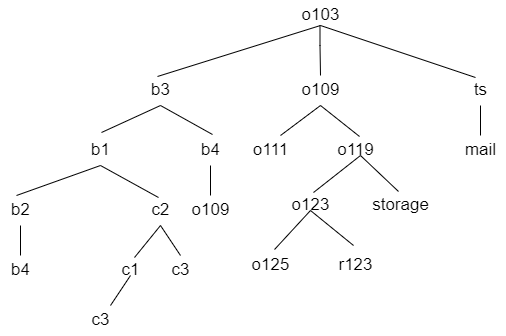
\includegraphics[width = 90mm,scale=0.90]{images/tree2.png}
	\vspace*{-3mm}
	\caption{Το δένδρο του προβλήματος για το ρομπότ.}
	\label{fig:mesh1}
\end{figure}
\vspace{1mm}

\noindent \bf 1. Αναζήτηση πρώτα σε πλάτος:\,\normalfont Για να βρούμε τη σειρά με την οποία εξάγονται οι κόμβοι από το σύνορο στη περίπτωση της αναζήτησης πρώτα σε πλάτος διασχίζουμε το δένδρο του Σχήματος~\ref{fig:mesh1} όπως στον αλγόριθμο {\lat BFS}. Έτσι, η σειρά με την οποία βγαίνουν οι κόμβοι σε αυτή την περίπτωση είναι η εξής: {\lat o103, b3, o109, ts, b1, b4, o111, o119, mail, b2, c2, o109, o123, storage, b4, c1, c3, o125, r123}.
\vspace{2mm}

\noindent \bf 2. Αναζήτηση πρώτα σε βάθος:\,\normalfont Εδώ οι κόμβοι εξάγονται με την ίδια σειρά που επισκεφτόμαστε τους κόμβους στο δένδρο κατά τον αλγόριθμο {\lat DFS}. Έτσι, έχουμε την εξής σειρά: {\lat o103, b3, b1, b2, b4, c2, c1, c3, c3, b3, b4, o109, o109, o111, o119, o123, o125, r123}.
\vspace{2mm}

\noindent \bf 3. Αναζήτηση πρώτα σε βάθος με επαναληπτική εκβάθυνση:\,\normalfont  Σε αυτή την περίπτωση εφαρμόζουμε διαδοχικά στα επίπεδα 1,2,3, 4, 5 τον αλγόριθμο {\lat DFS} μέχρις ότου να φτάσουμε στον κόμβο στόχου {\lat r123}. Έτσι η σειρά σε αυτή την περίπτωση δίνεται μέσω της ακολουθίας: {\lat o103, b3, o109, ts, o103, be, b1, b4, o109, o111, o119, ts, mail, o103, b3, b1, b2, c2 , b4, o109, o109, o111, o119, o123, storage, ts, mail, o103, b3, b1, b2, b4, c2, c1, c3, b4, o109, o109, o111, o119, o123, o125, r123}.
\vspace{2mm}

\noindent \bf 4. Άπληστη αναζήτηση πρώτα στον καλύτερο με ευρετική συνάρτηση την $h$:\normalfont\, Σε αυτή την περίπτωση διαλέγεται ο κόμβος με τη μικρότερη τιμή στη συνάρτηση $h$ για να εξαχθεί. Έτσι έχουμε την εξής σειρά: {\lat o103, b3, b1, b1, c2, c3, b2, b4, o109, o119, o123, r123}.
\vspace{2mm}

\noindent \bf 5. $A^*$ με ευρετική συνάρτηση την $h$:\, \normalfont Σε αυτή την περίπτωση επιλέγεται ο κόμβος του συνόρου με τη μικρότερη τιμή στην ποσότητα $f(n)+h(n)$. Η σειρά που προκύπτει με αυτή την προσέγγιση είναι η εξής: {\lat o103, b3, b1, c2, c1, b4, c3, ts, o109, o119, o123, r123.}
\vspace{2mm}

\section*{Πρόβλημα 4}

\noindent (α) Για να ορίσουμε ένα πρόβλημα αναζήτησης με μαθηματικό τρόπο θα πρέπει να προσδιορίσουμε τα εξής 4 στοιχεία:
\begin{itemize}
    \item[1.] Αρχική κατάσταση
    \item[2.] Συνάρτηση διαδόχων: ζευγάρια της μορφής $\langle \text{ενέργεια, διάδοχος} \rangle$.
    \item[3.] Έλεγχος στόχου και
    \item[4.] Κόστος διαδρομής.
\end{itemize}
\noindent Για το πρόβλημα μεταφοράς των πακέτων από το ρομπότ στα διάφορα δωμάτια έχουμε τα εξής:
\begin{itemize}
    \item[-] Ως \bf αρχική κατάσταση \normalfont θεωρούμε ένα ζευγάρι της μορφής $\pair{\text{δωμάτιο}}{\text{κατάσταση πακέτων}}$, όπου η πρώτη συνιστώσα υποδηλώνει το δωμάτιο στο οποίο βρίσκεται το ρομπότ και η δεύτερη συνιστώσα περιέχει ένα \emph{λεξικό ({\lat dictionary})} με \emph{κλειδιά {\lat (keys)}} τα πακέτα προς παράδοση και \emph{τιμές ({\lat values)}} τις ενδείξεις «1» σε περίπτωση που έχει παραδοθεί το πακέτο και «0» σε αντίθετη περίπτωση. Έτσι, με βάση τα παραπάνω η αρχική κατάσταση περιγράφεται με απ' το ζευγάρι που η πρώτη συνιστώσα είναι το δωμάτιο «{\lat mail}» και η κατάσταση των πακέτων έχουν όλα την ένδειξη «0», πράγμα το οποίο σημαίνει ότι δεν έχει παραδοθεί κανένα πακέτο στον προορισμό του.
    
    \item[-] Τώρα με βάση τους παραπάνω ορισμούς η \bf κατάσταση στόχου \normalfont είναι ένα ζευγάρι της μορφής $\pair{\text{δωμάτιο1}}{\text{κατάσταση πακέτων}}$ όπου η πρώτη συνιστώσα αντιστοιχεί σε ένα οποιοδήποτε δωμάτιο μπορεί να βρεθεί το ρομπότ και η δεύτερη στο λεξικό με τιμές την ένδειξη «1» για όλα τα κλειδιά, πράγμα το οποίο υποδηλώνει ότι το ρομπότ βρίσκεται στο δωμάτιο «δωμάτιο1» έχοντας παραδώσει όλα τα πακέτα. Να σημειώσουμε εδώ ότι δε χρειάζεται να απαιτήσουμε απ' το ρομπότ να βρίσκεται στην τελική κατάσταση στο δωμάτιο «{\lat mail}» γιατί αν το ρομπότ βρεθεί σε ένα οποιοδήποτε δωμάτιο έχοντας παραδώσει όλα τα πακέτα τότε το μόνο που έχουμε να κάνουμε για λάβουμε υπ'όψιν την επιστροφή του ρομπότ στο δωμάτιο «{\lat mail}» είναι να προσθέσουμε στο κόστος διαδρομής την απόσταση επιστροφής στο δωμάτιο «{\lat mail}» (βλέπε και παρακάτω στον ορισμό του κόστους διαδρομής).
    
    \item[-] Το ρομπότ μπορεί να εκτελεί δύο \bf ενέργειες: \normalfont 1) Μετακίνηση από το $\text{δωμάτιο1}$ στο $\text{δωμάτιο}2$ για παράδοση πακέτου (παράδοση) και 2) μετακίνηση από το $\text{δωμάτιο}1$ στο $\text{δωμάτιο}2$ για παραλαβή πακέτου (παραλαβή). Έτσι, η \bf συνάρτηση διαδόχων \normalfont περιγράφεται μέσω της αντιστοίχισης
    \[
    \triple{\text{δωμάτιο1}}{\text{ενέργεια}}{\text{δωμάτιο2}}\mapsto \pair{\text{δωμάτιο2}}{\text{κατάσταση πακέτων}},
    \]
    η οποία ερμηνεύεται ως «μετακίνηση από το δωμάτιο1 στο δωμάτιο2 μέσω της ενέργειας "ενέργεια"», όπου $\text{ενέργεια}\in \{\text{παράδοση},\text{παραλαβή}\}.$
    
    \item[-] Τέλος, για το \bf κόστος διαδρομής \normalfont θεωρούμε την απόσταση από την αρχική κατάσταση μέχρι οποιαδήποτε κατάσταση στόχου όπου έχουν παραδοθεί όλα τα πακέτα συν την απόσταση απ' το τελευταίο δωμάτιο που βρίσκεται το ρομπότ μέχρι το δωμάτιο «{\lat mail}».
\end{itemize}
\vspace{2mm}

\noindent (β) Μια \bf παραδεκτή ευρετική συνάρτηση \normalfont  για το πρόβλημα είναι η εξής: Για μια κατάσταση $\underbrace{\pair{\text{δωμάτιο1}}{\text{κατάσταση πακέτων}}}_{n}$ μπορούμε να ορίσουμε 
\begin{align*}
h(n) &= \text{«Η απόσταση από το κόμβο } n \text{ μέχρι τον κόμβο } n' \text{ όπου έχουν παραδοθεί όλα τα πακέτα}\\
&+ \text{την απόσταση που απαιτείται για να μεταφερθεί το ρομπότ από το δωμάτιο του κόμβου } n'\\
&\quad \, \, \text{μέχρι το δωμάτιο «{\lat mail}»»}.
\end{align*}
\noindent Πιο αναλυτικά, στη περίπτωση που στην κατάσταση $n$ υπάρχουν $k$ υπολοιπόμενα πακέτα προς παράδοση, τότε αυτά περιγράφονται από ζευγάρια της μορφής $\pair{\text{δωμάτιο}1k}{\text{δωμάτιο}2k}$, όπου για το πακέτο $1\leq i \leq k$ πρέπει το ρομπότ να το παραλάβει απ' το $\text{δωμάτιο}1k$ και να το παραδώσει στο $\text{δωμάτιο}2k$. Με αυτό τον συμβολισμό έχουμε ότι
\[\tag{4.1}\label{eq:4.1}
h(n) = \sum_{j=1}^k\text{απόσταση}\left(\text{δωμάτιο}1j,\, \text{δωμάτιο}2j\right) + \text{απόσταση}\left(\text{δωμάτιο}2k,\text{{\lat mail}}\right),
\]
\noindent όπου με τον συμβολίσμό $\text{απόσταση}\left(\text{δωμάτιο}1j,\, \text{δωμάτιο}2j\right)$ εννοούμε την απόσταση μεταξύ των δωματίων $\text{δωμάτιο}1j$ και $\text{δωμάτιο}2j$. Η συνάρτηση $h$ είναι παραδεκτή αφού για κάθε κατάσταση $n$ που βρίσκεται το ρομπότ σίγουρα θα διανύσει αυτές τις αποστάσεις για να παραδώσει όλα τα υπολοιπόμενα πακέτα και αυτό συμβαίνει διότι το ρομπότ μπορεί να μεταφέρει μόνο ένα πακέτο τη φορά.
\vspace{2mm}

\section*{Πρόβλημα 5}

\noindent Όπως γνωρίζουμε η αμφίδρομη αναζήτηση στη περίπτωση που και οι δύο αναζητήσεις χρησιμοποιούν {\lat BFS} είναι πλήρης και βέλτιστη όταν ο παράγοντας διακλάδωσης $b$ είναι πεπερασμένος. Τώρα, έχουμε τα εξής:
\vspace{2mm}

\noindent (α) \bf Αναζήτηση πρώτα σε πλάτος και αναζήτηση περιορισμένου βάθους:\,\normalfont Τώρα στην περίπτωση που η προς τα πίσω αναζήτηση γίνεται με αναζήτηση περιορισμένου βάθους τότε ο αλγόριθμος αμφίδρομης αναζήτησης \bf είναι πλήρης\normalfont, όταν ο παράγοντας διακλάδωσης είναι πεπερασμένος αλλά εν γένει \bf όχι βέλτιστος. \normalfont Το ότι είναι πλήρης όταν ο παράγοντας διακλάδωσης είναι πεπερασμένος προκύπτει απ' το γεγονός ότι η αναζήτηση κατα πλάτος πάντα καταλήγει σε μια λύση. Έτσι, ακόμα και αν δεν συναντηθούν οι δύο αναζητήσεις σε κάποιο σημείο ο προς τα εμπρός αλγόριθμος αναζήτησης που γίνεται πρώτα κατά πλάτος κάποια στιγμή θα βρει τον στόχο και η αμφίδρομη αναζήτηση θα τερματίσει επιστρέφοντας μια λύση. Παρ'όλα αυτά, ο αλγόριθμος δεν είναι βέλτιστος εφόσον στη περίπτωση που συναντηθούν τα μονοπάτια η προς τα πίσω αναζήτηση μπορεί να ακολουθήσει ένα μη βέλτιστο μονοπάτι προς τη λύση και τότε το τελικό μονοπάτι που θα προκύψει θα είναι μη βέλτιστο. Ακόμα και αν δεν συναντηθούν τα μονοπάτια, μόνο η προς τα εμπρός αναζήτηση μας εγγυάται ότι θα τερματίσει ο αλγόριθμος. Όμως, γνωρίζουμε ότι η αναζήτηση πρώτα κατά πλάτος δεν επιστρέφει πάντα (εκτός αν είναι ομοιόμορφα τα κόστη) μια βέλτιστη λύση.
\vspace{2mm}

\noindent (β) \bf Αναζήτηση με επαναληπτική εκβάθυνση και αναζήτηση περιορισμένου βάθους:\,\normalfont Σε αυτή την περίπτωση η αναζήτηση πάλι \bf είναι πλήρης \normalfont (όταν το $b$ πεπερασμένο) αλλά \bf όχι βέλτιση. \normalfont Το ότι είναι πλήρης προκύπτει απ' το γεγονός ότι η αναζήτηση με επαναληπτική εκβάθυνση επιστρέφει πάντα μια λύση, και έτσι, ακόμα και αν δεν συναντηθούν οι δύο αναζητήσεις η προς τα εμπρός αναζήτηση θα φτάσει κάποια στιγμή στον στόχο. Ο λόγος που ο αλγόριθμος δεν είναι βέλτιστος είναι ο ίδιος όπως και στην περίπτωση (α).
\vspace{2mm}

\noindent (γ) \bf $A^*$ και αναζήτηση περιορισμένου βάθους: \normalfont Σε αυτή την περίπτωση η αμφίδρομη αναζήτηση \bf είναι πλήρης αλλά όχι βέλτιστη. \normalfont Στη περίπτωση που ευρετική συνάρτηση είναι παραδεκτή, η ακόμα καλύτερα συνεπής, τότε η προς τα εμπρός αναζήτηση που γίνεται με $A^*$ θα τερματίσει κάποια στιγμή έχοντας βρει μια λύση. \normalfont Τώρα, για να δούμε ότι δεν είναι βέλτιστος, αυτό προκύπτει απ' το γεγονός ότι η αναζήτηση περιορισμένου βάθους μπορεί να δημιουργήσει ένα μη βέλτιστο μονοπάτι προς τη λύση και αυτό να συναντηθεί με κάποιο κόμβο της εμπρόσθιας αναζήτησης δίνοντας συνολικά ένα μη βέλτιστο μονοπάτι για τη λύση.
\vspace{2mm}

\noindent (δ) \bf $Α^*$ και $A^*$: \normalfont Σε αυτή την περίπτωση, αν τουλάχιστον μια απ' τις δύο ευρετικές συναρτήσεις που χρησιμοποιούν οι επιμέρους αναζητήσεις είναι παραδεκτή ή συνεπής και ισχύει ότι $b<\infty$, τότε η αμφίδρομη αναζήτηση θα βρει μια λύση, και έτσι είναι πλήρης σε αυτή την περίπτωση. Τώρα, αν μια τουλάχιστον απ' τις δύο συναρτήσεις δεν είναι παραδεκτή, τότε ο αλγόριθμος μπορεί να βρει τη βέλτιστη λύση. Αν και οι δύο είναι παραδεκτές ή συνεπείς, τότε ο αλγόριθμος θα βρει τη βέλτιστη λύση.
\vspace{2mm}

\noindent Στον παρακάτω πίνακα συνοψίζουμε όλα τα παραπάνω.

\begin{center}
\captionof{table}{Ο έλεγχος της συνέπειας για την ευρετική συνάρτηση $h$} \label{tab:2} 
\begin{tabular}{ C{1in} C{1in} C{1in} C{1in} C{1in}}\toprule[1.5pt]
\bf Κριτήριο & Περίπτωση (α) & Περίπτωση (β) & Περίπτωση (γ) & Περίπτωση (δ)\\
Πλήρης{\lat ;} & Ναι$^\alpha$ & Ναι$^\alpha$ & Ναι$^{\alpha,\beta}$ & Ναι$^{\alpha,\gamma}$\\
Βέλτιστη{\lat ;} & Όχι & Όχι & Όχι & Ναι$^{\alpha,\delta}$ \\
\bottomrule[1.5pt]
\end{tabular}
\end{center}
\noindent Οι επιφυλάξεις που εμφανίζονται στον πίνακα είναι οι εξής: $^\alpha$ ο παράγοντας διακλάδωσης είναι πεπερασμένος, $^\beta$ Η ευρετική συνάρτηση είναι παραδεκτή, $^\gamma$ τουλάχιστον μια απ' τις δύο συναρτήσεις είναι παραδεκτή, $^\epsilon$ και οι δύο ευρετικές συναρτήσεις είναι παραδεκτές.
\vspace{2mm}

\noindent Τέλος, όσον αφορά την αποδοτικότητα του ελέγχου για το αν οι δύο αναζητήσεις συναντιούνται σε κάποιον κόμβο αυτό μπορεί να γίνει με τη χρήση ενός πίνακα κατακερματισμού για το σύνορο μιας εκ των δύο αναζητήσεων. Για παράδειγμα, στην {\lat Python} αυτή η δομή μπορεί να αναπαρασταθεί από ένα σύνολο ({\lat set}) όπου ο έλεγχος αν υπάρχει ένα στοιχείο στο σύνολο ή όχι γίνεται με $O(1)$.

\end{document}
